\section{Проектрирование общей части}
Прежде чем приступать к непосредсвенной реализации индивидуальной части курсовой работы, была разработана
общая часть проекта. В неё входит диаграмма вариантов использования и концептуальная диаграмма классов.

Диаграмма прецедентов (Use case diagram, диаграмма вариантов использования)~-- диаграмма, на которой отражены отношения, 
существующие между экторами и прецедентами.
Основная задача~-- представлять собой единое средство, дающее возможность заказчику, конечному пользователю и разработчику совместно
обсуждать функциональность и поведение системы.

Сущности, с которыми взаимодействует система в процессе своей работы, называются экторами, причем каждый эктор ожидает, 
что система будет вести себя строго определенным, предсказуемым образом. В качестве экторов могут выступать человек или 
другая система, подсистема или класс, которые представляют нечто вне сущности.
Прецедент (use-case)~-- описание отдельного аспекта поведения системы с точки зрения пользователя.
В данном проекте диаграмма прецедентов выглядит так:

\begin{figure}[h]
\centering
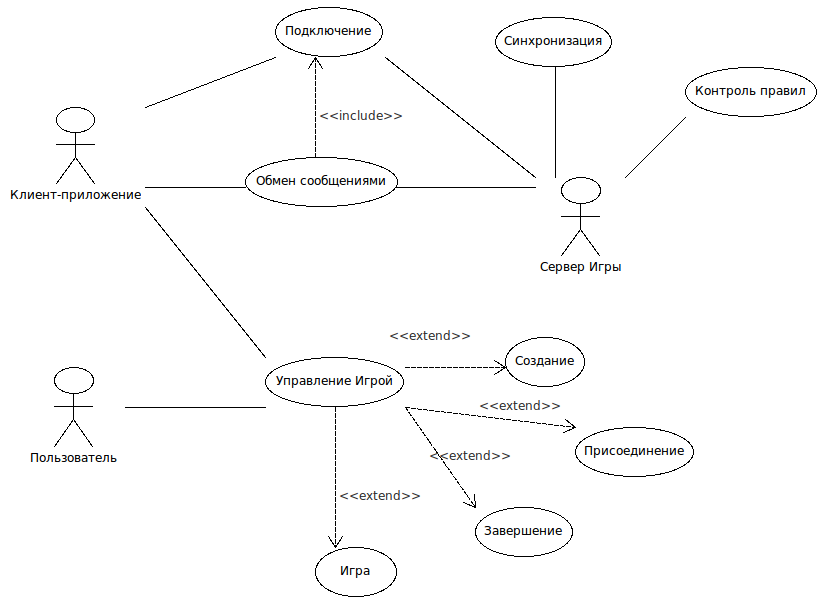
\includegraphics[width=18cm]{images/use.png}
\caption{Диаграмма прецедентов}
\label{fig.0}
\end{figure}

На данной диаграмме видно, что взаимодействие игроков и все их действия осуществляются через сервер игры, который
занимается синхронизацией действий игроков(т.е. чтобы игроки видели перемещения кораблей друг друга)
и проверкой соответсвия их действий правилам игры. Под ролью пользователя на данной диаграмме понимается 
человек, который взаимодействует с данным приложением(графическим интерфрейсом программы).
Клиенту должны быть доступны возможности создания и завершения игры, а так же непосредсвенный процесс. Все это вмете объединено под единым вариантом икпользования, названным <<Управление Игрой>>. Контроль произведенных операций осуществляется отдельной сущностью(сервером). Третий эктор несет вспомогательнуя роль и является своеобразным посредником между пользователем и сервером. У него должен иметься интерфейс как графический, так и для общения с серверной частью. Исходя из выше сказанного, была построенна концептуальная часть диаграммы классов.

\begin{figure}[h]
\centering
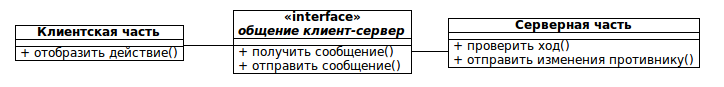
\includegraphics[width=17cm]{images/class.png}
\caption{Диаграмма классов а)}
\label{fig.1}
\end{figure}

Проанализировав данную диаграмму, было принято решение её детализировать, выделив на ней отдельные классы те части проекта, которые непосредственно должны реализовывать описанный интерфейс. Стоит обратить внимание, что такие классы должны быть как в клиентской, так в серверной частях.

\begin{figure}[h]
\centering
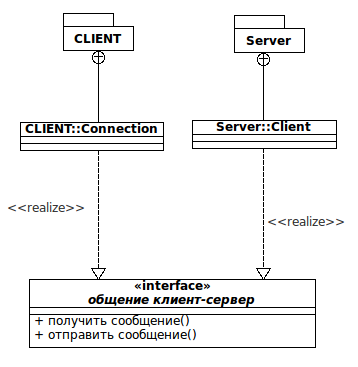
\includegraphics[width=9cm]{images/class1.png}
\caption{Диаграмма классов б)}
\label{fig.2}
\end{figure}

% на рисунке ~\ref{fig.1}
\endinput
